\documentclass[letter,11pt]{article}

\usepackage{amsfonts}
\usepackage{amsmath}
\usepackage{amssymb}
\usepackage[brazilian]{babel}
\usepackage{enumerate}
\usepackage[T1]{fontenc}
%\usepackage[ansinew,latin1]{inputenc}
\usepackage[utf8x]{inputenc}
\usepackage{multicol}
\usepackage{graphicx}
\setlength\columnseprule{0.5pt}

\newtheorem{exer}{Exercício}
\newtheorem{teo}{Teorema}

\newcommand{\var}{Var}
\newcommand{\E}{\mathbb{E}}

\newcommand{\mat}[1]{\mbox{\boldmath{$#1$}}}

\usepackage[letterpaper,top=3cm, bottom=2cm, left=2.5cm, right=2.5cm]{geometry}

\begin{document}

%\thispagestyle{empty}
\begin{center}{ \Large MAT02026 - Inferência B }\end{center}

\begin{center}
{\large  \sc Gabarito Lista 3 - Testes MP e UMP, função poder e TRV}
\end{center}
\vspace{5mm}

%%%%%%%%%%%%%%%%%%%%%%%%%%%%%%%%%%%%%%%%%%%%%%%%%%%%%%%%%%%%%%%%%%%%%%%%%%%%%%%
% Exercicios da lista 1 Marcia... incluir???
\begin{exer} \rm
% Suponha que a proporção $p$ de itens defeituosos, em uma grande população de itens,
% seja desconhecida. Deseja-se testar as seguintes hipóteses $H_0 : p = 0,2$ versus
% $H_1 : p \neq 0,2$. Considere que uma amostra aleatória de 20 itens seja retirada
% desta população e denote $Y$ = número de itens defeituosos na amostra. O seguinte
% procedimento de teste será usado: Rejeitar $H_0$ se $Y \geq 7$ ou $Y \leq 1$.
\begin{enumerate}[a)]
%   \item Determine a funcão poder deste teste.
%   \item Calcule o valor da função poder para os seguintes pontos
%   $p = \{0, 0.1, 0.2, 0.3, 0.4, 0.5, 0.6, 0.7, 0.8, 0.9, 1\}$. Faça o gráfico.
%   \item Determine o tamanho do teste, ou seja, o valor de $\alpha = \sup_{\theta
%   \in\Theta_0} \beta(\theta)$.
\item $\beta(p)$ inclui as seguintes expressões:
$$
\sum_{y=7}^{20}  {20 \choose y}p^y(1-p)^{20-y} \qquad e \qquad \sum_{y=0}^1  {20 \choose y}p^y(1-p)^{20-y}
$$


\item $\beta(p) = \{1, 0.39, 0.16, 0.4, 0.75, 0.94, 0.99, 1, 1, 1, 1\}$. 

\item

\end{enumerate}
\end{exer}


\begin{exer} \rm
% Seja $X_1, \ldots, X_{10} $ uma amostra aleatória de tamanho $n = 10$ tal que
% $X_i \sim Bernoulli(\theta)$ onde $P(X_i = 1) = \theta = 1 - P(X_i = 0)$.
% Considere as hipóteses $H_0 : \theta \leq 1/2$ contra $H_1 : \theta > 1/2$.
% Assuma a seguinte regra de teste: Rejeitar $H_0$ se $\sum X_i \geq 6$.
\begin{enumerate}[a)]
%   \item Determine a função poder do teste.
%   \item Calcule a função poder para os seguintes pontos $p = \{0, 0.1, 0.2, 0.3, 0.4, 0.5, 0.6, 0.7, 0.8, 0.9, 1\}$. Faça o gráfico.
%   \item Determine o tamanho do teste, ou seja, o valor de $\alpha = \sup_{\theta \in\Theta_0} \beta(\theta)$.
 \item $\beta(p)$ inclui a expressão:
$$
\sum_{x=6}^{10}  {10 \choose x}\theta^x(1-\theta)^{10-x} 
$$
 
 \item $\beta(p) = \{0, 0, 0.01, 0.05, 0.17, 0.38, 0.63, 0.85, 0.97, 0.99, 1\}$. 
 
 \item 0,38

\end{enumerate}
\end{exer}


\begin{exer} \rm
% Considere a variável aleatória $X$ com a seguinte densidade $f(x) = \theta x^{\theta-1}I_{(0,1)}(x)$. Para testar as hipóteses $H_0 : \theta \leq 1$ versus $H_1: \theta > 1$, uma única observação $(X_1)$ foi amostrada e o seguinte critério de rejeição foi adotado: rejeitar $H_0$ se $X_1 > 1/2$.
\begin{enumerate}[a)]
%   \item Encontre a função poder deste teste.
%   \item Determine o tamanho do teste.

\item $\beta(\theta)=1-\frac{1}{2^\theta}$
 \item 0.5
\end{enumerate}
\end{exer}
%%%%%%%%%%%%%%%%%%%%%%%%%%%%%%%%%%%%%%%%%%%%%%%%%%%%%%%%%%%%%%%%%%%%%%%%%%%%%%%
% Lista 3 Marcia

% \begin{exer} \rm Seja $X_1, \ldots, X_n$ variáveis aleatórias da distribuição Weibull $(\alpha, \beta)$, 
% 
% $$
% f(x/\alpha, \beta)=\beta \alpha x^{\alpha-1}\exp(-\beta x^\alpha), \quad \alpha >0, \beta>0.
% $$
% 
% A função de log-verossimilhança é dada por 
% 
% $$
% L(\alpha, \beta/x) = n\log\beta + n\log \alpha + (\alpha-1) \sum_{i=1}^n \log X_i -\beta\sum_{i=1}^n X_i^\alpha.
% $$
% 
% Essa distribuição é alguma vezes parametrizada em termo de $\alpha$. Depois de substituir $\beta$ por seu estimador de máxima verossimilhança $\hat{\beta}=n/\sum_{i=1}^n X_i^\alpha$ o profile da log-verossimilhança pode ser escrito como 
% 
% $$
% L(\alpha, \hat{\beta}(\alpha)/x) = n\log n -n \log (\sum_{i=1}^n X_i^{\alpha}) + (\alpha-1) \sum_{i=1}^n \log X_i + n\log \alpha -n.
% $$
% 
% Gere artificialmente, no software R, uma amostra de $n=25$ observações da distribuição Weibull com $\alpha=1.5$ e $1/\beta^\alpha=2$. Utilizando o método de Newton-Raphson com valor inicial $\alpha^{(0)}=0.5$, indique os cálculos e valores encontrados nas primeiras 5 iterações. Quais os valores de $\alpha^{(5)}$ e $\hat{\beta}(\alpha^{(5)})$?
% 
% Utilize a função optim do R para estimar $\alpha$ e $\beta$.
% \end{exer}


% \begin{exer} \rm Considere a equação
% $$
% g(\theta)= \theta^2 -4
% $$
% 
% Dado o ponto inicial $\theta^{(0)}=3$, utilize o método de Newton-Raphson para encontrar a raiz. Mostre os cálculos e indique os valores até o 4 passo. 
% \end{exer}


% \begin{exer} \rm Seja $X_1, \ldots, X_6$ uma amostra aleatória de uma distribuição Exponencial de parâmetro $\lambda$. Dado que os valores observados na amostra foram  $\textbf{x}=\{0.031; 0.05; 0.029; 0.318; 0.754; 0.327\}$. 
% 
% \begin{enumerate}[a)]
% \item Através do método de Newton-Raphson calcule o estimador $\tilde{\lambda}$, faça 5 iterações e utilize como ponto inicial o valor 3. 
% 
% \item Calcule o estimador de máxima verossimilhança.
% 
% \item Utilize o software R para gerar uma amostra de tamanho 250 de uma distribuição Exponencial de parâmetro $\lambda=5$. Refaça as letras (a) e (b) para essa nova amostra.
% 
% \end{enumerate}
% \end{exer}


\begin{exer} \rm 
% Suponha que $X_1, \ldots, X_n$ é uma amostra aleatória tal que $X_i \sim \mbox{Bernoulli}(\theta)$. Calcule $\lambda(X)$ e determine o critério de rejeição para o TRV (Teste da Razão de Verossimilhanças) considerando as hipóteses $H_0: \theta \leq \theta_0 $ versus $H_0: \theta > \theta_0 $, em que $\theta_0$ é um valor conhecido especificado pelo pesquisador.

Se $\theta_0< \overline{X}$, então 
$$ \lambda(X)=\left(\frac{\theta_0}{\overline{X}}\right)^{\sum X_i}\left(\frac{1-\theta_0}{1-\overline{X}}\right)^{n-\sum X_i}. $$
\end{exer}


\begin{exer} \rm 
% Seja $X_1, \ldots, X_n$ uma amostra obtida a partir da distribuição Exponencial com parâmetro $\theta$.

\begin{enumerate}[a)]
% \item Encontre o TRV para testar $H_0: \theta = 1$ versus $H_1: \theta \neq 1$.
% 
% \item Se uma amostra de tamanho $n=5$ observasse os seguintes valores $\textbf{x}=\{0.8; 1.3; 1.8; 0.9; 1\}$, qual seria a sua conclusão se escolhermos a constante $c=0.5$.
\item Rejeitar $H_0$ se $
((\overline{X})^n\exp\{n(1-\overline{X})\})< c $ para algum $c \in (0,1)$

\item Não rejeitar $H_0$.
\end{enumerate}
\end{exer}


\begin{exer} \rm 
% Seja $X_1, \ldots, X_n$ uma amostra aleatória da distribuição $N(\mu_x, 9)$ e considere $Y_1, \ldots, Y_m$ uma amostra aleatória da distribuição $N(\mu_y, 25)$. Assuma que essas duas amostras são independentes.

\begin{enumerate}[a)]
% \item Encontre o TRV para $H_0: \mu_x=\mu_y$ versus $H_1: \mu_x\neq \mu_y$. Dica: Determine a distribuição de $\overline{X}-\overline{Y}$.

% \item Se você observar $n=9$, $\sum_{i=1}^9 x_i=3.4$, $m=16$, $\sum_{i=1}^{16} y_i=4.3$. Qual seria a sua decisão considerando $c=0.5$.
\item Rejeitar $H_0$ se $\exp\{-\frac{1}{2V}W^2\}< c$, onde $V=\frac{9}{n}+\frac{25}{m}$, $W=\overline{X}-\overline{Y}$ e $c\in (0,1)$.

\item Não rejeitar $H_0$
\end{enumerate}
\end{exer}


\begin{exer} \rm 
% Seja $X_1, \ldots, X_n$ uma amostra aleatória da distribuição Gama$(3, \lambda)$. Encontre o TRV para as hipóteses $H_0:\lambda=\lambda_0$ versus $H_1: \lambda \neq \lambda_0$, onde $\lambda_0$ é um valor positivo e especificado pelo pesquisador.
Se $\lambda_0 < \hat{\lambda}$ rejeitamos $H_0$ se $\left(\left(\frac{\lambda_0}{\hat{\lambda}}\right)^{3n}\exp{(\hat{\lambda}-\lambda_0)\sum X_i}\right)< c$, onde $c \in (0,1)$ e $\hat{\lambda}$ é o EMV de $\lambda$.
\end{exer}


\begin{exer} \rm 
% Seja $X_1, \ldots, X_n$ uma amostra aleatória da densidade
% $$
% f(x/\theta)=\frac{2x}{\theta}I_{(0, \theta]}(x),
% $$
% 
% onde $\theta>0$.  Encontre o TRV para as hipóteses $H_0:\theta\geq\theta_0$ versus $H_1: \theta < \theta_0$, onde $\theta_0$ é um valor positivo e especificado pelo pesquisador.
Se $\theta_0 \geq x_{(n)}$ rejeitamos $H_0$ se $\left(\frac{x_{(n)}}{\theta_0}\right) < c$ onde $c \in (0,1)$ e $x_{(n)}=\max\{X_1, \ldots, X_n\}$.
\end{exer}

%%%%%%%%%%%%%%%%%%%%%%%%%%%%%%%%%%%%%%%%%%%%%%%%%%%%%%%%%%%%%%%%%%%%%%%%%%%%%%%
% lista 4 Marcia

\begin{exer} \rm 
% Seja $X_1, \ldots, X_n$ uma amostra aleatória da variável $X \sim $ Geométrica$(\theta)$.

% \begin{enumerate}[a)]
% \item Encontre o TRV para as hipóteses $H_0: \theta=\theta_0$ contra $H_1: \theta \neq \theta_0$.
% 
% \item Encontre o teste uniformemente mais poderoso (UMP) para testar $H_0: \theta=\theta_0$ versus $H_1: \theta=\theta_1$, em que $\theta_0<\theta_1$ são especificados pelo pesquisador.
% 
% \item  Encontre o teste UMP para $H_0: \theta=0.3$ versus $H_1: \theta=0.5$.
% 
% \item Dado o teste UMP calculado na letra (c), considere que $n=5$ e $\alpha=0.04$, qual o critério de rejeição? Qual o erro tipo II? Se a amostra observada fosse $x=\{4,5,3,2,5\}$ qual a sua decisão?
% 
% \item Gere artificialmente, no software R, uma amostra de $n= 100$ de uma distribuição geométrica com parâmetro $\theta=0.5$.  Dado o teste UMP calculado na letra (b) e $\alpha=0.04$, qual o critério de rejeição? Qual o erro tipo II? Compare com o resultado encontrado na letra (d).
% 
% \end{enumerate}
\end{exer}
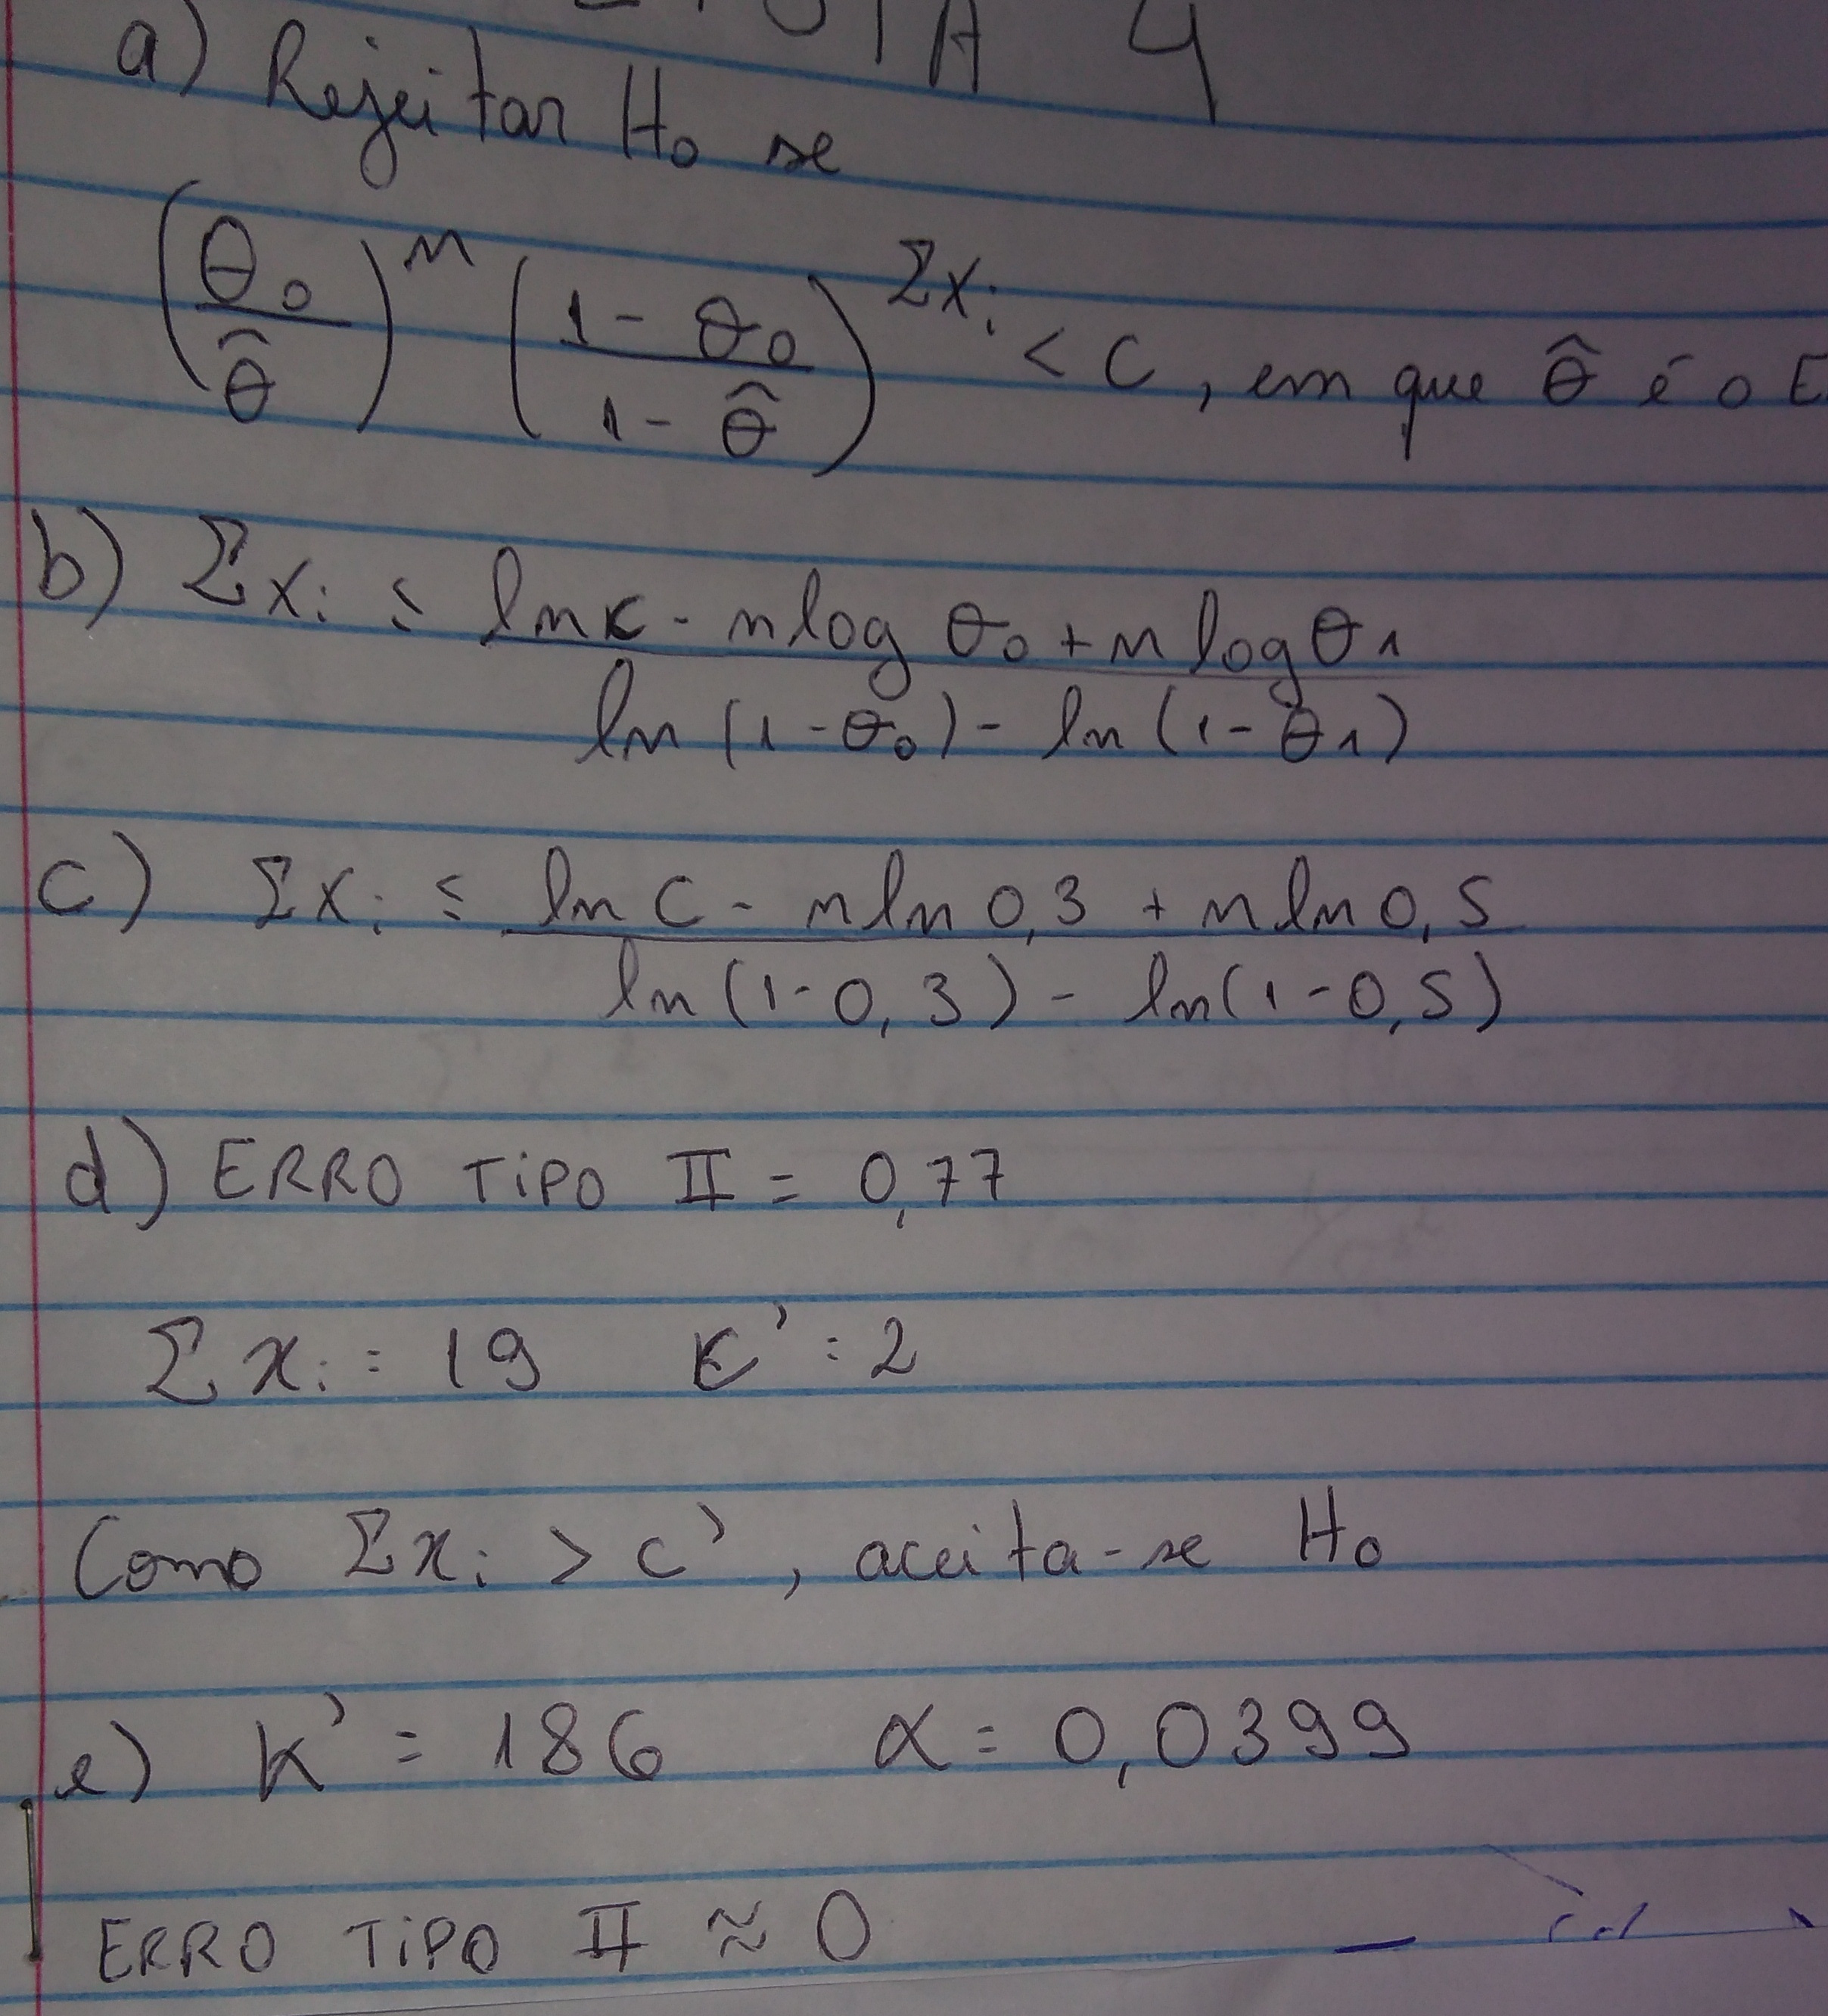
\includegraphics[scale=0.1]{Ex9_gabarito}


\begin{exer} \rm 
% Seja $X_1, \ldots, X_n$ uma amostra aleatória de tamanho $n$ da distribuição $N(\mu, 1)$.
% \begin{enumerate}[a)]
% \item Encontre o teste UMP para as hipóteses $H_0: \mu=0$ contra $H_1: \mu=1$.
% 
% \item Suponha que $n=9$ e $\alpha=0,05$. Qual é a região crítica do teste obtido em (a).
% 
% \item Faça o gráfico da função poder da letra (b).
% \end{enumerate}
\end{exer}
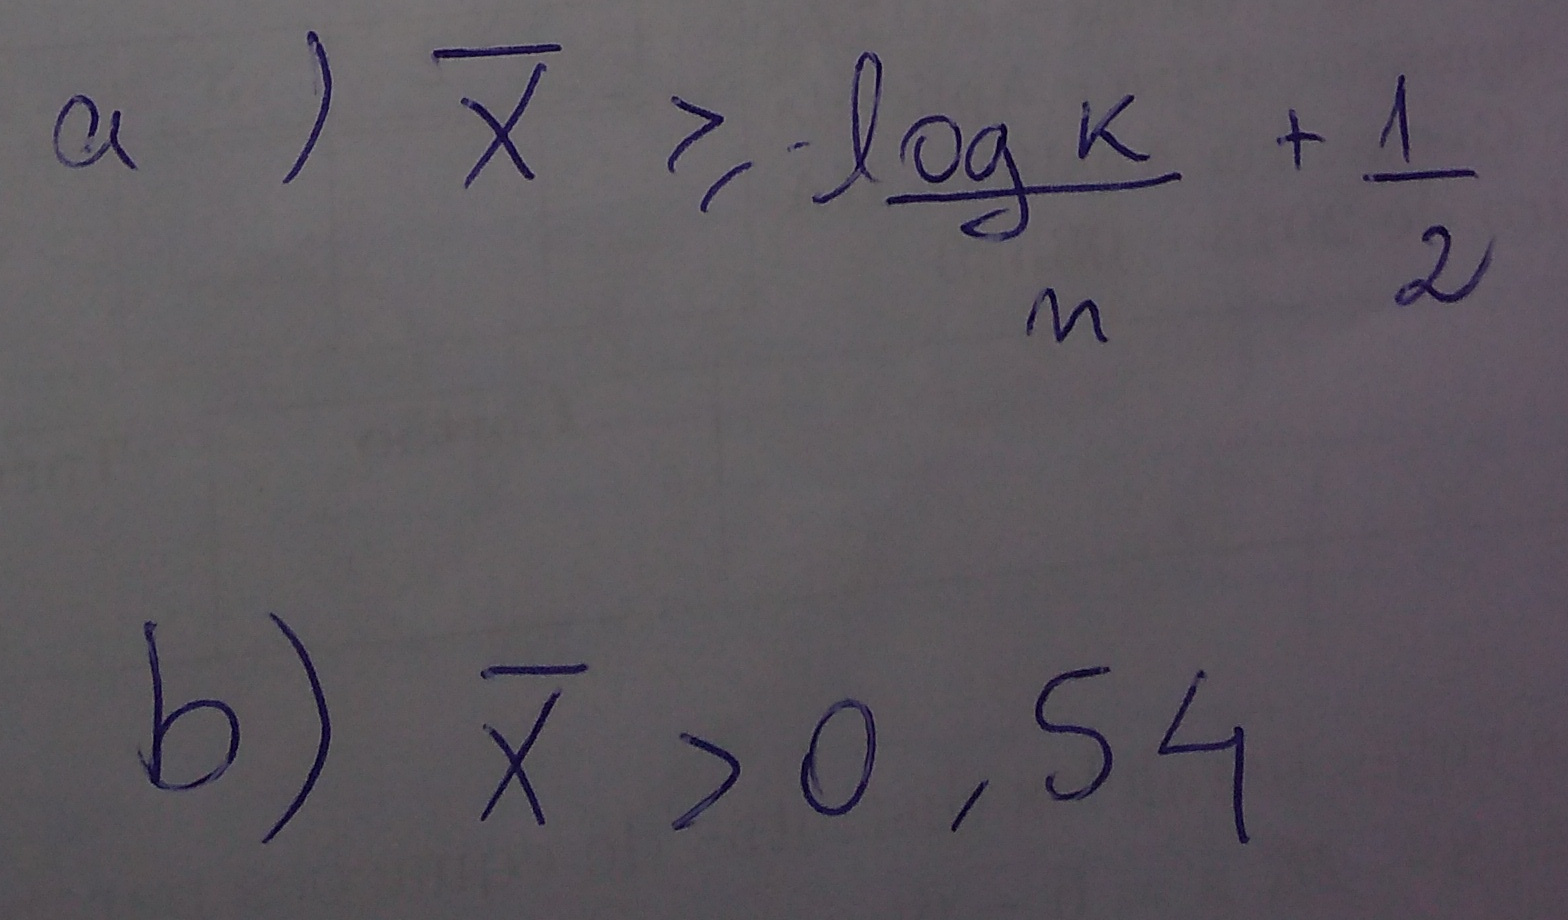
\includegraphics[scale=0.1]{Ex10_gabarito}


\begin{exer} \rm 
% Seja $X_1, \ldots, X_n$ uma amostra aleatória da variável $X$ com a seguinte função densidade:
% 
% $$
% f(x/\theta)=\theta x^{\theta-1} I_{(0,1)}, \mbox{ em que } \theta>0.
% $$
% 
% \begin{enumerate}[a)]
% \item O teste mais poderoso para $H_0: \theta=1$ versus $H_1: \theta=2$ rejeitará $H_0$ se $[\sum_{i=1}^n -\log (x_i) \leq a]$ onde $a$ é uma constante. Mostre este resultado.
% 
% \item Sendo $n=2$ e $\alpha=[1-\log(2)]/2$ qual seria a região crítica? Dica: se $X \sim$ Beta($\theta$, 1) então $-\log(X)\sim$ Exp($\theta$).
% \end{enumerate}
\end{exer}
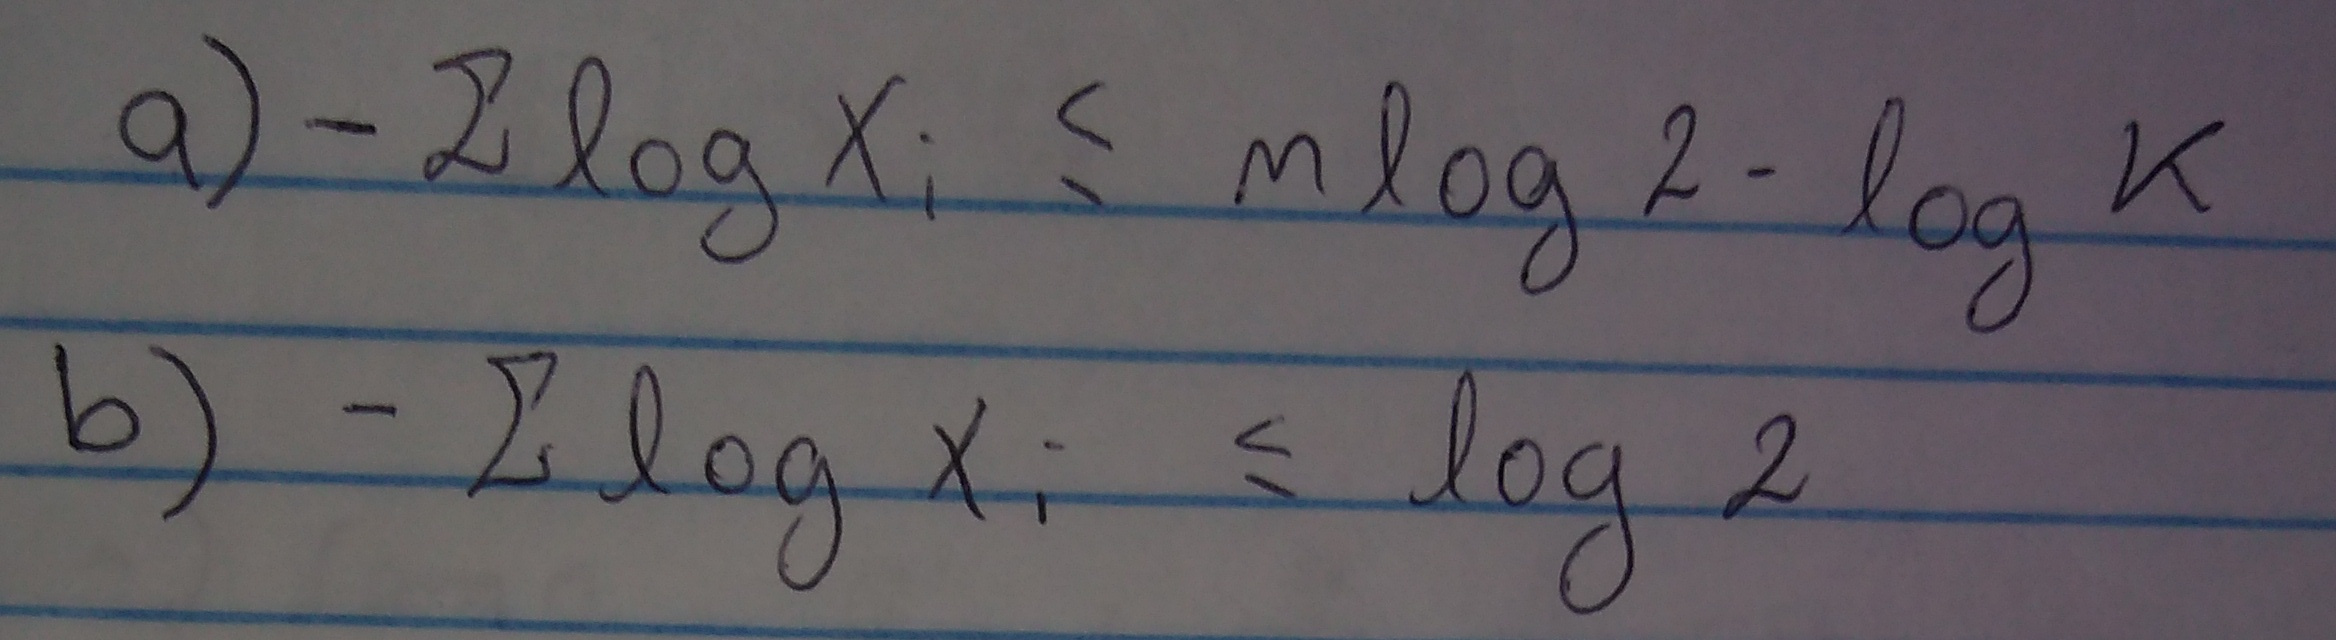
\includegraphics[scale=0.1]{Ex11_gabarito}


\begin{exer} \rm 
% Seja $X_1, \ldots, X_n$ uma amostra aleatória obtida da distribuição Poisson($\theta$). Encontre o teste UMP para as hipóteses $H_0: \theta=\theta_0$ versus $H_1: \theta=\theta_1$, considere que $\theta_0 < \theta_1$
\end{exer}
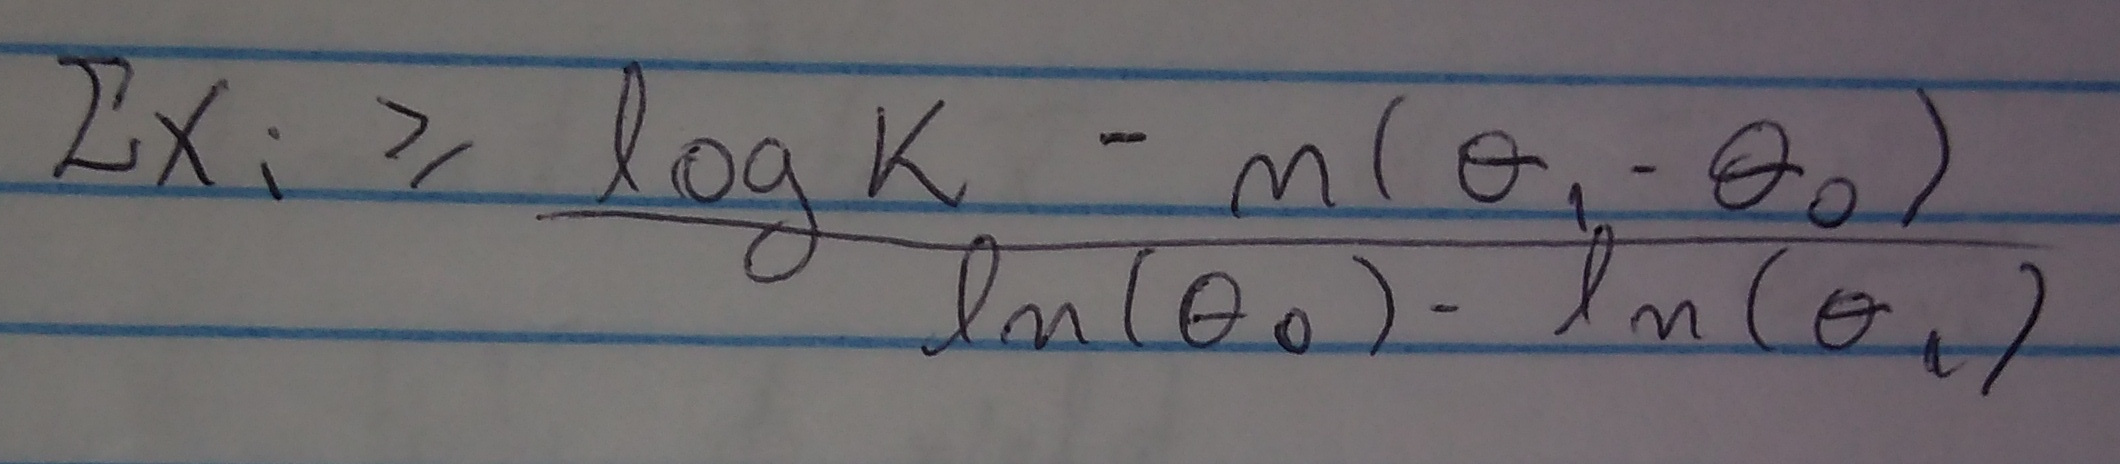
\includegraphics[scale=0.1]{Ex12_gabarito}


\begin{exer} \rm 
% Seja $X_1, \ldots, X_n$ uma amostra aleatória obtida da distribuição $N(0, \sigma^2)$.
% \begin{enumerate}[a)]
% \item Encontre o teste UMP para $H_0:\sigma^2=\sigma_0^2$ versus $H_1:\sigma^2=\sigma_1^2$. Considere que $\sigma_0^2< \sigma_1^2$.
% 
% \item Sendo $\sigma_0^2=1$, $\sigma^2_1=2$, $n=2$ e $\alpha=0.05$, qual seria a região crítica? 
% 
% 
% \item Gere artificialmente, no software R, uma amostra de $n= 10$ da distribuição normal com parâmetros $(\mu=0, \sigma^2=2)$.  Dado o teste UMP calculado na letra (a), as hipóteses $\sigma_0^2=1$, $\sigma^2_1=2$ e $\alpha=0.04$, qual o critério de rejeição? Qual o erro tipo II? Qual a sua decisão dado essa amostra?
% 
% \item Refaça o item anterior, mas utilize uma amostra de tamanho $n=100$.  Compare com o resultado encontrado na letra (c).
% 
% \end{enumerate}
\end{exer}
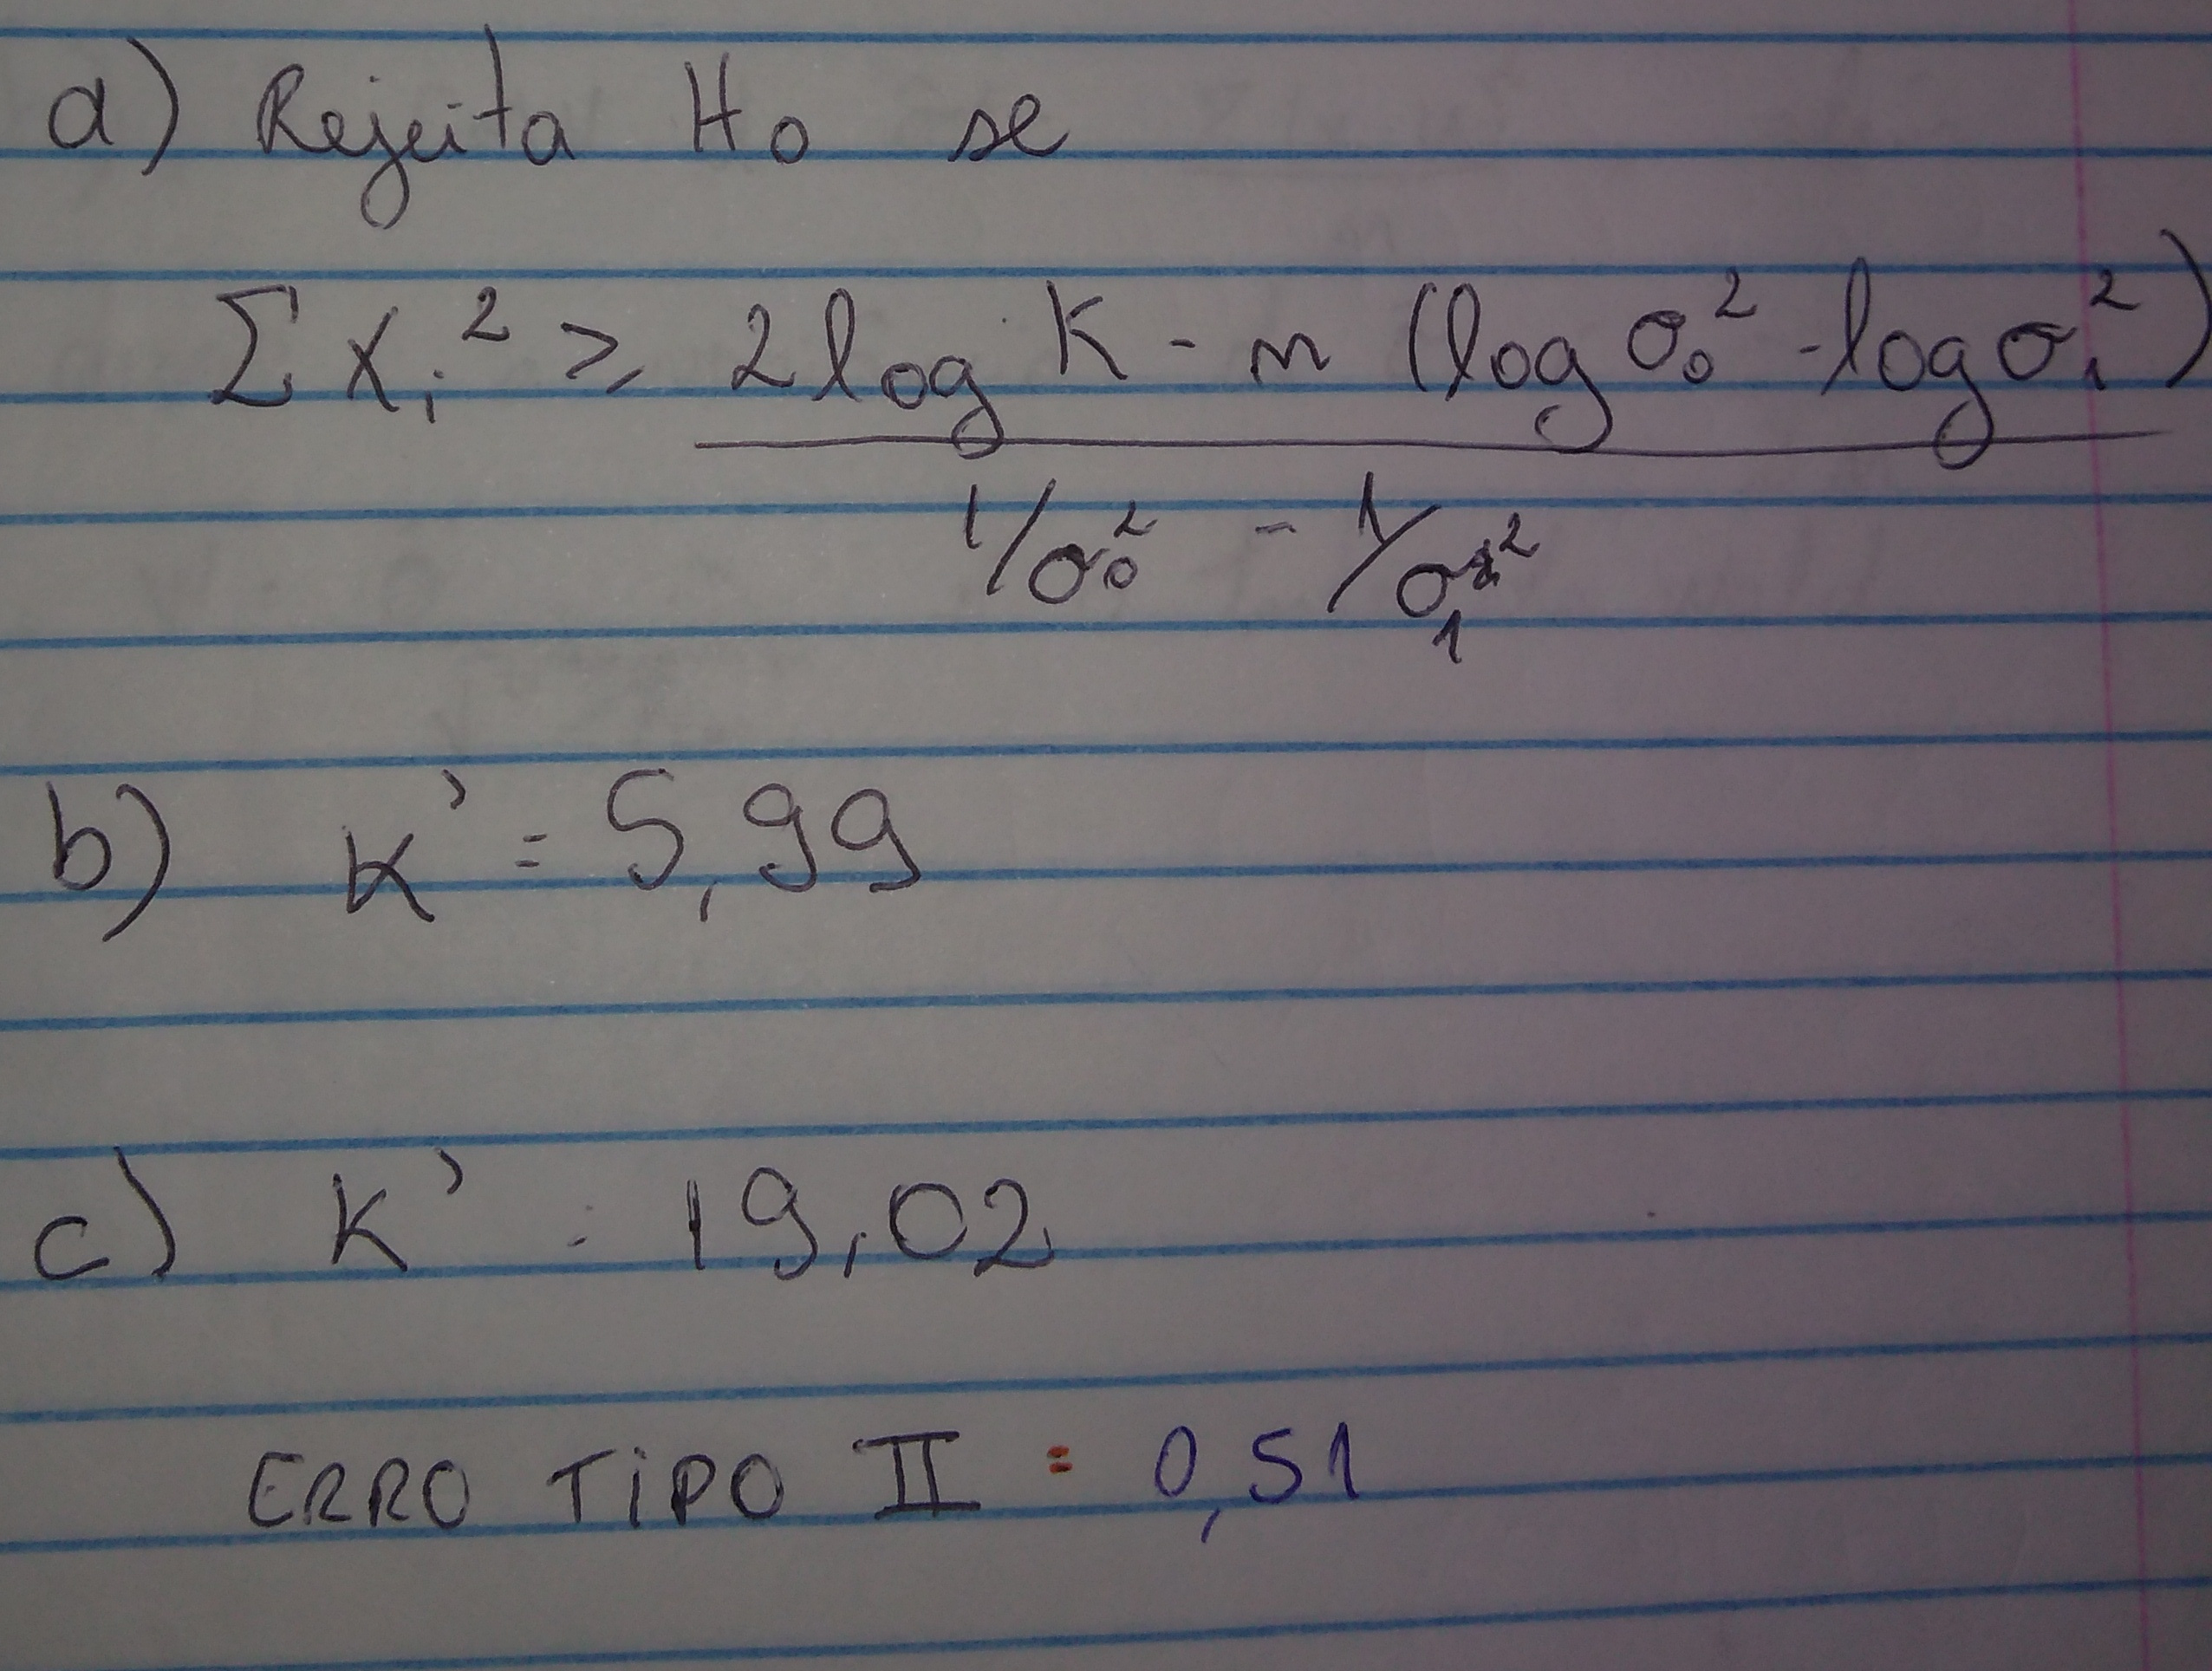
\includegraphics[scale=0.1]{Ex13_gabarito}


\begin{exer} \rm %O que é 'valor $p$'?
\end{exer}


\begin{exer} \rm %O que é nível descritivo amostral? 
\end{exer}


\begin{exer} \rm %O que é nível de significância?
\end{exer}
%%%%%%%%%%%%%%%%%%%%%%%%%%%%%%%%%%%%%%%%%%%%%%%%%%%%%%%%%%%%%%%%%%%%%%%%%%%%%%%
% lista 4 Marcio

% \begin{exer} \rm  %(Pg 3 e 4 apostila) -tem resposta
% Uma caixa contém 2 moedas. Uma apresenta cara com probabilidade 0,5 (equilibrada) e a outra apresenta cara com probabilidade 0,6 (viesada). Uma delas é escolhida aleatoriamente e lançada 3 vezes. Deseja-se saber se a moeda selecionada é a equilibrada ou a viesada.
% 
% \begin{enumerate}[a)]
% \item Defina um teste para decidir entre $H_0:\theta=0.5$ e $H_1:\theta=0.6$.
% \item Calcule as probabilidades de erro tipo I e II.
% \end{enumerate}
% \end{exer}
% 
% 
% \begin{exer} \rm  %(8.1 Casella and Berger) -tem resposta
%  Em 1000 lançamentos de uma moeda, foram observadas 560 caras e 440 coroas. É razoável assumir
% que a moeda é equilibrada?
% \end{exer}
% 
% 
% \begin{exer} \rm %(8.2 Casella and Berger) -tem resposta
%  Em uma determinada cidade o número de acidentes com automóveis em dado ano segue a distribuição de Poisson.
%  Nos últimos anos a média do número de acidentes por ano foi 15, e este ano foi 10. É correto afirmar que o
% número de acidentes está diminuindo?
% \end{exer}
% 

\begin{exer} \rm 
% %(8.13 Casella and Berger) - tem resposta
%  Seja $X_1,\ldots,X_n$  i.i.d. uniforme($\theta,\theta+1$). Para testar $H_0:\theta =0$ versus (vs.) $H_1:\theta > 0$, temos dois testes concorrentes:
% 
%  $$\phi_1(X_1): \mbox{ Rejeita } H_0 \mbox{ se } X_1> 0.95,$$
%  $$\phi_2(X_1): \mbox{ Rejeita } H_0 \mbox{ se } X_1+X_2> C,$$

\begin{enumerate}[a)]
% \item Encontre o valor de $C$ para o qual $\phi_2$ tenha o mesmo tamanho  que $\phi_1$.
% 
% \item    Calcule a função poder de cada teste. Desenhe a função poder de cada teste.
% 
% \item $\phi_2$ é mais poderoso que $\phi_1$?
% 
% \item Mostre como encontrar um teste que tenha o mesmo tamanho de $\phi_2$, mas que seja mais poderoso que $\phi_2$.

\item 
O tamanho de $\phi_1$ pode ser obtido diretamente por 

\[\alpha=P(X_1>0.95)=0.05.\]


Para calcular o tmanho de $\phi_2$ precisamos encontrar a distribuição de $Z=X_1+X_2$, sendo que $X_1\sim U(0,1)$ e $X_2\sim U(0,1)$. Observe na figura (histograma), que foi gerada com o código 
\begin{verbatim}
# Gerando uniformes
x1=runif(100000,0,1)
x2=runif(100000,0,1)
z=x1+x2
hist(z,freq=F,breaks=60,main=expression("Z =" ~ X[1]+X[2] ~ ",  " ~ X[1] ~ "~U(0,1) " ~ ",  
                                        " ~ X[2] ~ "~U(0,1) "), ylab=expression(f[Z](z)))
\end{verbatim}

que a distribuição de $Z$ em questão é uma distribuição triangular.

\begin{center}
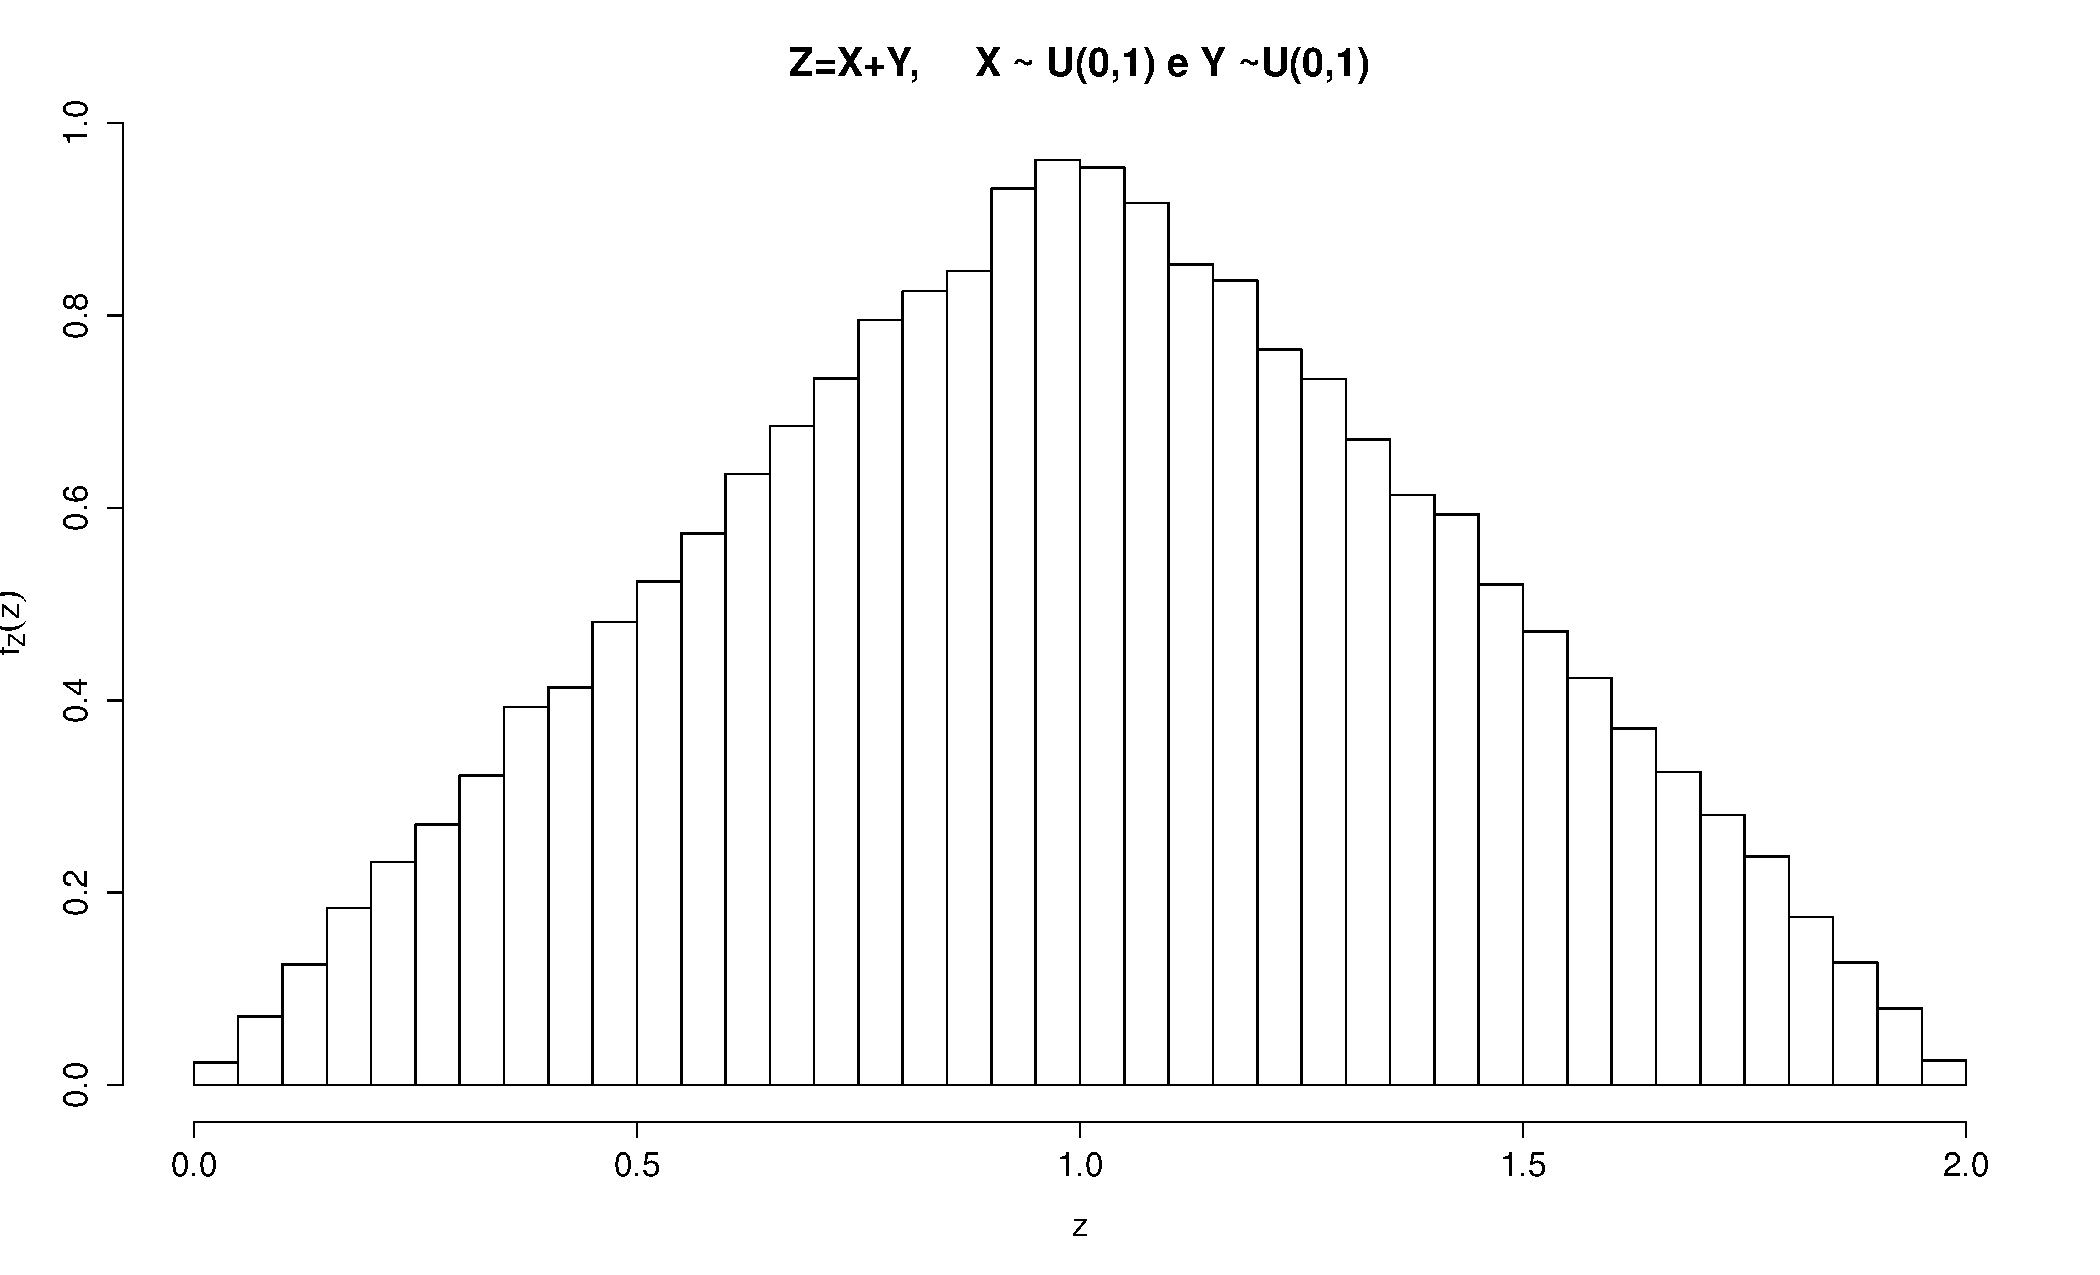
\includegraphics[scale=0.4]{sumunif.pdf} 
\end{center} 

Podemos usar a convolução para obter a densidade de $Z$. Assim, para $0\leq z\leq 2$

\begin{eqnarray*}
f_Z(z)&=&f_{X_1+X_2}(z)=
\int_{-\infty}^{\infty}f_x(x)f_Y(z-x)dx\\
&=&\int_{0}^{1}f_x(x)f_Y(z-x)dx
=\int_{0}^{1}f_Y(z-x)dx\\
&=&\begin{cases}
 \int_{0}^{z} f_Y(z-x)dx & \mbox{ se } 0\leq z< 1\\
 \int_{z-1}^{1} f_Y(z-x)dx & \mbox{ se } 1\leq z\leq 2\\
\end{cases}\\
&=&\begin{cases}
 z & \mbox{ se } 0\leq z< 1\\
 2-z & \mbox{ se } 1\leq z< 2\\
 0 & \mbox{ caso contrário.}
\end{cases}
\end{eqnarray*} 

Assim, para encontrar $C$ tal que $P(X_1+X_2 > C)=0.05$ é razoável/necessário assumir que $1\leq C\leq 2$. Logo

\[P(X_1+X_2>C]=P(Z>C)=\int_{C}^{1}(2-z)dz=\frac{(2-C)^2}{2}.\]


Segue que $\alpha=0.05$,  C= 1.68.%Encontre o valor de $C$ para o qual $\phi_2$ tenha o mesmo tamanho  que $\phi_1$.

\item    %Calcule a função poder de cada teste. Desenhe a função poder de cada teste.

\[\beta_1(\theta)=P_\theta(X_1>0.95)=\begin{cases}
 0 & \mbox{ se } \theta\leq -0.05\\
 \theta+0.05 & \mbox{ se } -0.05< \theta\leq 0.95\\
 1 & \mbox{ se } 0.95<\theta.
\end{cases}\]

Para encontrar a função poder do teste $\phi_2$ precisamos calcular a distribuição/densidade de $Z=X_1+X_2$ em que $X_i\sim U(\theta,\theta+1)$. Usando o fato que a densidade da soma $X_1+X_2$ é uma triangular entre $2\theta$ e $2\theta+2$, podemos escrevê-la como

\begin{eqnarray*}
f_Z(z)
&=&\begin{cases}
 z-2\theta & \mbox{ se } 2\theta \leq z< 2\theta+1\\
 2\theta +2-z & \mbox{ se } 2\theta+1\leq z <2\theta+ 2\\
 0 & \mbox{ caso contrário.}
\end{cases}
\end{eqnarray*} 


 
\[\beta_2(\theta)=P_\theta(X_1+X_2>C)
=\begin{cases}
0 & \mbox{ se } \theta \leq C/2-1\\
 (2\theta +2-C)^2/2 & \mbox{ se } C/2-1 < \theta \leq (C-1)/2\\
 1-(C-2\theta)^2/2 & \mbox{ se } (C-1)/2< \theta \leq C/2\\
 0 & \mbox{ se } C/2<\theta.
\end{cases}\]

Assuma que C=1.68 e faça os gráficos.

%=\begin{cases}
% 0 & \mbox{ se } \theta\leq -0.05\\
% \theta+0.05 & \mbox{ se } -0.05< \theta\leq 0.95\\
% 1 & \mbox{ se } 0.95<\theta.
%\end{cases}\]

\item  Observe nos gráfico que em algumas regiões o $\phi_2$   tem mais poder que o $\phi_1$ e em outras regiões o contrário acontece.
%$\phi_2$ é mais poderoso que $\phi_1$?

\item %Mostre como encontrar um teste que tenha o mesmo tamanho de $\phi_2$, mas que seja mais poderoso que $\phi_2$.

Uma opção é rejeitar $H_0:\theta=0$ também quando $X_1>1$ ou $X_2> 1$. Nesse caso o tamanho continua o mesmo do $\phi_2$ mas você rejeita em mais situações. Então seria mais poderoso que $\phi_2$.


\end{enumerate}
\end{exer}


% \begin{exer} \rm  %(ex 3 mae3-l6 listas da net) -tem resposta
%  Seja $X_1,\ldots,X_n$  a.a. de uma v.a. $X$ com função de densidade dada por
% 
% \[f(x)=\theta x^{\theta-1},\,\,\,\,0<x<1,\,\,\,\theta> 0.\]
% 
% \begin{enumerate}[a)]
% \item  Mostre que o teste mais poderoso para testar  $H_0:\theta =1$ vs. $H_1:\theta = 2$ rejeita $H_0$, se e somente se, $\sum_{i=1}^n -\log x_i\leq a$, em que $a$ é uma constante.
% 
% \item Sendo $n=2$ e $\alpha=(1-\log 2)/2$, qual é a região crítica?
% \end{enumerate}
% \end{exer}


\begin{exer} \rm %(ex 3 mae3-l6 listas da net) -tem resposta
 % Seja $X_1,\ldots,X_n$ a.a. de uma v.a. $X$ com função de densidade $N(0,\sigma^2)$.

\begin{enumerate}[a)]
\item %Encontre o teste uniformemente mais poderoso (UMP) para testar $H_0:\sigma^2 =\sigma_0^2 $ vs. $H_1:\sigma^2 > \sigma_0^2 $
O teste mais poderoso para esse teste alternativo será o de região crítica dada por

\[A^*=\left\{{\bf x};\frac{L_1({\bf x})}{L_0({\bf x})}\geq k\right\}\].

\[\frac{L_1}{L_0}\geq k \Leftrightarrow  \sum x_i^2\geq \log\left[k(\sigma_1^2/\sigma_0^2)^{n/2}\right]\left(\frac{1}{2\sigma_0^2}-\frac{1}{2\sigma_1^2}\right)^{-1}=c \]

Assim, o teste MP acima terá região crítica dada por 

\[A^*=\left\{\sum x_i ^2 \geq c\right\}\].

Como o teste acima vale para qualquer valor de $\sigma_1^2$ , ele  também será o teste UMP. 



\item %Seja $\alpha = 0.05$, $n = 9$ e $\sigma_0^2=9$.
 %Faça o gráfico da função poder.
 
 Observe que \[\sum \left(\frac{X_i}{3}\right)^2\sim\chi^2_{(9)}\]
 
 e 
 
 \[\alpha = P_{H_0}\left(\sum X_i^2 \geq c\right)=P_{H_0}\left( \sum\left(\frac{X_i}{3}\right)^2\geq \frac{c}{9}\right)\]
 
 Dessa forma, basta encontrarmos $c/9$ com o comando  $qchisq(0.95,9).$

 \[\frac{c}{9}=16.91898 \rightarrow c=152.2708.\]
 
 Segue que  a função poder é dada por \[\beta(\sigma^2)=P\left(X\geq \frac{152.2708}{\sigma^2}\right)\]
 em que $X\sim\chi^2_{(9)}$.
 
 Use o R para fazer os gráficos. 
 \end{enumerate}
\end{exer}


\begin{exer} \rm  %(8.12 Casella and Berger) -tem resposta
% Para amostras de tamanho $n=1,4,16,64,100$ de uma população normal com média $\mu$ e variância conhecida $\sigma^2$, faça o gráfico da função poder dos seguintes testes da razão de verossimilhança (TRV's). Tome $\alpha=0.05$.
\begin{enumerate}[a)]
\item %$H_0:\mu\leq 0$  vs. $H_1:\mu>0$.


Fazendo a razão de verossimilhanças encontramos que rejeita-se $H_0$ se $\overline{x}>\frac{c\sigma}{\sqrt{n}}$. Para $\alpha=0.05$ temos que $c=1.645$.

\[\beta(\mu)=P\left(\frac{\overline{X}-\mu}{\sigma/\sqrt{n}}>1.645-\frac{\mu}{\sigma/\sqrt{n}}\right)=P\left(Z>1.645-\frac{\sqrt{n}\mu}{\sigma}\right)\]

\item %$H_0:\mu= 0$  vs. $H_1:\neq 0$
Nesse caso rejeita-se $H_0$ se $|\overline{x}|>\frac{c\sigma}{\sqrt{n}}$. Para $\alpha=0.05$ temos que $c=1.96$.

\[\beta(\mu)=P\left(-1.96-\frac{\sqrt{n}\mu}{\sigma}\leq Z\leq 1.96+\frac{\sqrt{n}\mu}{\sigma}\right)\]

\end{enumerate}
\end{exer}


\begin{exer} \rm  %(8.5 Casella and Berger) -tem resposta
%  Uma a.a. $X_1,\ldots,X_n$ é retirada de uma população Pareto com densidade
% 
% $$f(x|\theta,\nu)=\frac{\theta\nu^\theta}{x^{\theta+1}}I_{\nu,\infty}(x),\,\,\,\theta>0,\,\,\,\nu>0.$$

\begin{enumerate}[a)]
\item %Encontre os EMV's de $\theta$ e $\nu$.
$\hat{\nu}=x_{(1)}$ e \[\hat{\theta}=\frac{n}{\log\left(\prod x_i/x_{(1)}^n\right)}=\frac{n}{T}\]
\item % Mostre que o TRV
%$$H_0: \theta=1,\,\,\nu\,\,\mbox{desconhecido},\,\,\,\,\,\,\,vs\,\,\,\,\,\,\, H_1: \theta\neq 1,\,\,\nu\,\,\mbox{desconhecido},$$
%tem região critica da forma $\{x:T(x)\leq c_1\,\,ou\,\,T(x)\geq c_2\}$, em que $0<c_1<c_2$ e $$T=\log \left[ \frac{\prod_{i=1}^{n}X_i}{(\min_i X_i)^n}\right].$$
\[\lambda({\bf x})=\frac{L_1({\bf x})}{L_0({\bf x})}=\left(\frac{T}{n}\right)^n e^{-T+n}.\]

Observe que $\frac{\partial}{\partial T}\log \lambda({\bf x})=(T/n) -1. $ Assim,  $\lambda({\bf x})$ é crescente para $T\leq n$ e decrescente para $T\geq n$. Ou seja, existe um $c_1$ e um $c_2$ tal que  $\lambda({\bf x})$ é grande se $T\geq c_1$ ou $T\leq c_2$.
\end{enumerate}
\end{exer}


\begin{exer} \rm  %(8.6 Casella and Berger) -tem resposta
% Suponhamos que temos duas amostras de variáveis aleatórias independentes: $X_1\ldots,X_n$ são exp($\theta$) e $Y_1\ldots,Y_n$ são exp($\mu$). Encontre o TRV de $H_0:\theta=\mu$ vs. $H_1:\theta\neq \mu$.
% 
%\begin{enumerate}[a)]
%\item Encontre o TRV de $H_0:\theta=\mu$ vs. $H_1:\theta\neq \mu$.
%\item Mostre que o teste da parte a) pode ser baseado na estatística
%$$T=\frac{\sum X_i}{\sum X_i+\sum Y_i}.$$
%\item Encontre a distribuição de $T$ quando $H_0$ é verdadeira.
%
%\end{enumerate}
\end{exer}


\begin{exer} \rm  %(8.8 Casella and Berger) -tem resposta
% Um caso especial da família de distribuições \emph{normal} é quando a média e a variância são relacionadas, como por exemplo a família $N(\theta,a\theta)$. Se estamos interessados em testar esse relacionamento, independente do valor de $\theta$, nos deparamos com um problema chamado problema do parâmetro ``nuisance''.
% 
% \begin{enumerate}[a)]
% \item Encontre o TRV de $H_0:a=1$ vs. $H_1:a\neq 1$ baseado em uma amostra $X_1,\ldots,X_n$ de uma família $N(\theta,a\theta)$, em que $\theta$ é desconhecido.
% 
% \item  Um problema similar ocorre quando a família é $N(\theta,a\theta^2)$. Assim, se  $X_1,\ldots,X_n$ são i.i.d. $N(\theta,a\theta^2)$, quando $\theta$ é desconhecido, encontre o TRV de $H_0:a=1$ vs. $H_1:a\neq 1$.
% \end{enumerate}
\end{exer}


\end{document}